\documentclass[tikz,convert={density=150,size=600,outext=.png}]{standalone}
\usetikzlibrary{shapes, calc, arrows, fit, positioning, decorations, patterns, decorations.pathreplacing, chains, snakes}

\begin{document}
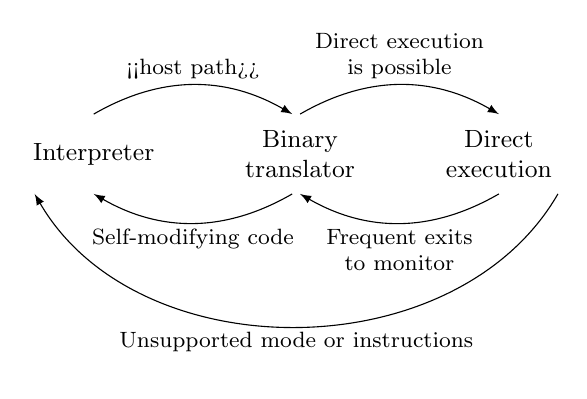
\begin{tikzpicture}[>=latex, font=\small, align=center, inner sep=2pt]
\node[minimum height = 1.cm] (interp) {Interpreter};
\node[minimum height = 1.cm, right = of interp] (bt) {Binary\\translator};
\node[minimum height = 1.cm, right = of bt] (dex) {Direct\\execution};

\begin{scope}[auto, font=\footnotesize,  text width = 3cm]
\draw[->] (interp.north) to[bend left] node {<<host path>>} ([xshift=-0.1cm] bt.north);
\draw[->] (bt.north) to[bend left] node {Direct execution\\is possible} (dex.north);

\draw[->] ([xshift=-0.1cm] bt.south) to[bend left] node {Self-modifying code} (interp.south);
\draw[->] (dex.south) to[bend left] node {Frequent exits\\to monitor} (bt.south);
\end{scope}

\draw[->] ([xshift=0.75cm] dex.south) to[bend left=60] node[auto] {\footnotesize Unsupported mode or instructions} ([xshift=-0.75cm] interp.south);
\end{tikzpicture}
\end{document}
